\documentclass[english, a4paper, oneside, onecolumn, openany,article]{memoir}
\usepackage{fix-cm,fixltx2e}
\usepackage{babel}  % babel: Hyphenation patterns and language specific strings
\usepackage{varioref}
\usepackage[colorlinks,linkcolor=black,urlcolor=black,citecolor=black]{hyperref}
\usepackage[colorinlistoftodos]{todonotes}
\usepackage[latin1]{inputenc}
\usepackage{graphicx}
\usepackage{listings}
\usepackage[square,numbers]{natbib}
\usepackage{url}
\usepackage{pslatex}
\usepackage{multirow}
\usepackage[T1]{fontenc}
\usepackage{eso-pic}
\usepackage{xcolor,calc}
\usepackage{pdfpages}
\newsubfloat{figure}
\usepackage{placeins} % gives me FloatBarrier
%Forhindrer floats i at flyde ind i næste afsnit
\let\oldsection=\section % gemmer den gamle definition
\renewcommand\section{\FloatBarrier\oldsection}

\makeatletter
\renewcommand\fps@figure{htbp} % Force figure placement
\renewcommand\fps@table{htbp}
\makeatother

% setup captions
\hangcaption
\changecaptionwidth
\captionwidth{9cm}


\title{Advanced Data Management - Assignment 2}
\author{S\o ren Bjerregaard Vrist\\ITU Copenhagen}

\begin{document}
\maketitle

\chapter{Part1 - Writes}
\section{Part1a}
The objective is to try to experiment with write performance of DB2. 
First the baseline performance of an EC2 small instance running Ubuntu 9.10 with
``out-of-the-box'' db2 is reported. After that I've tried different tuning knobs
to in someway affect the insert performance.

Overall was it hard to find basis for experimentation. What can be improved and
how? 

\subsection{Results}
All experiements has been done via a comprehensive list of bash scripts included
in the appendix. The ``setup.bash''(Appendix \ref{app:setup} script contains all the auxiliary
information needed when running the experiments, including snapshot and vmstat
output. As descriped in the log (Section \ref{log:probwrite}) the writes.py had
problems so I decided to use my own edition of writes.py \footnote{profwrites2.py -
Appendix \ref{app:prof}} for all the following experiments.


\subsubsection{Baseline}
The baseline (for me) is the defaults from writes.py (5 runs, 10 threads,
InsertN,$100.000$ writes, 1.000.000 tuples). 
\begin{itemize}
  \item 17.1 seconds.
\end{itemize}
Vmstat doesnt show that it is IO bound:
\begin{verbatim}
procs -----------memory---------- ---swap-- -----io---- -system-- ----cpu----
 r  b   swpd   free   buff  cache   si   so    bi    bo   in   cs us sy id wa
...
 1  0      0 107032   4232 1315788    0    0     0    28   63   32 38  0  0  0
 9  1      0  63144   4276 1317044    0    0   300    48  110  299 29  7  1  3
12  1      0  57296   4296 1318260    0    0    62   818  116 10326 30  9  0  0
12  1      0  57296   4304 1318260    0    0     0  1210  117 14254 30  8  0  0
 9  0      0  57296   4328 1318260    0    0     4  1070  103 13700 30  8  0  0
12  1      0  57296   4328 1318260    0    0     0  1136   96 14041 31  7  0  0
 7  0      0  56232   4340 1319292    0    0     2  1066  120 13615 30  9  1  0
10  1      0  53192   4348 1322356    0    0     0  1050  107 13204 30  8  0  0
11  1      0  49544   4360 1325940    0    0     2  1008  103 13377 28 10  0  0
 3  0      0  69824   4360 1325912    0    0    24   638   90 8580 25 13  0  0
10  1      0  49080   4376 1325976    0    0     0   398   81 5465 31  7  0  0
11  1      0  48320   4380 1325992    0    0     2   900  112 11977 27 11  0  0
13  1      0  47000   4384 1326048    0    0    26   950  111 12514 26 12  0  0
11  1      0  44116   4392 1316488    0    0   510  1012  138 12102 26 12  0  0
 2  1      0  49896   4428 1300924    0    0    10   960  117 11966 26 11  0  0
 7  1      0  44416   4436 1302568    0    0   115   982  115 12887 29  9  0  0
14  1      0  41832   4444 1293864    0    0     0   910  105 11997 25 12  0  0
 9  1      0  44712   4328 1289512    0    0    68   844  107 11655 30  8  0  0
...
\end{verbatim}
Around 1000 in the ``bo'' column. Block/s sent to device). 
When measuring disk performance 20-60.000 is possible.

\subsubsection{Threads}
Maybe concurrency could improve this?
(I expected that it would actually be best with as few threads as possible
because of the RR isolation level). Figure \ref{fig:part1athreads}\footnote{This
experiment was rerun after the AUTO\_COMMIT bug was found} confirms my
suspicion that fewer threads are beneficial (due to locking when RR insolation
level is used).
\begin{figure}
  \centering
  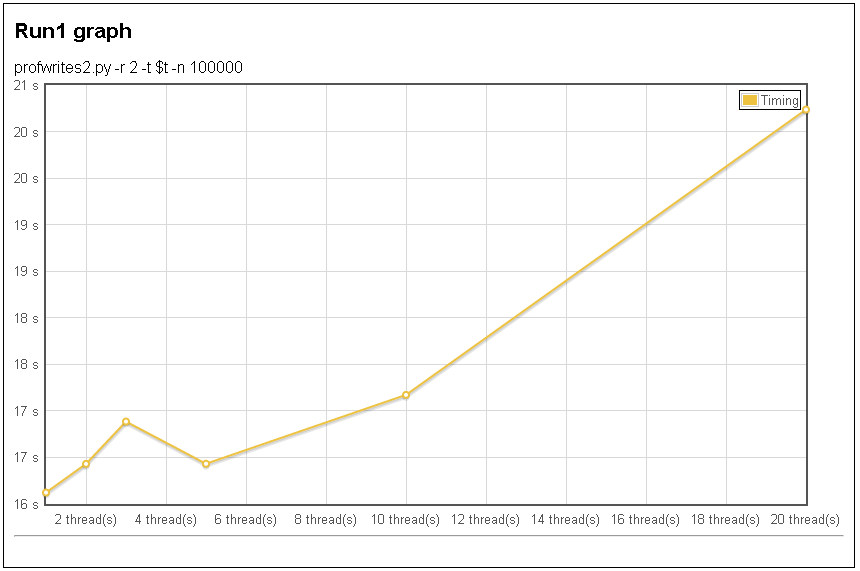
\includegraphics[width=12cm]{assignment2/run1}
  \caption[Insert performance]{Graph of insert timing for 100.000 rows(in one
  transaction) as a function of concurrency}\label{fig:part1athreads}
\end{figure}

\subsubsection{Indexes/primary key on table}
My next theory was that it might be because the time was spent maintaining index
integrity while inserting. The timing results can be seen in figure
\ref{fig:part1aindex1}. Concurrency still gives a penalty, but it is a couple of
seconds faster for all concurrency level without a private key (and thereby an
index).
\begin{figure}
  \centering
  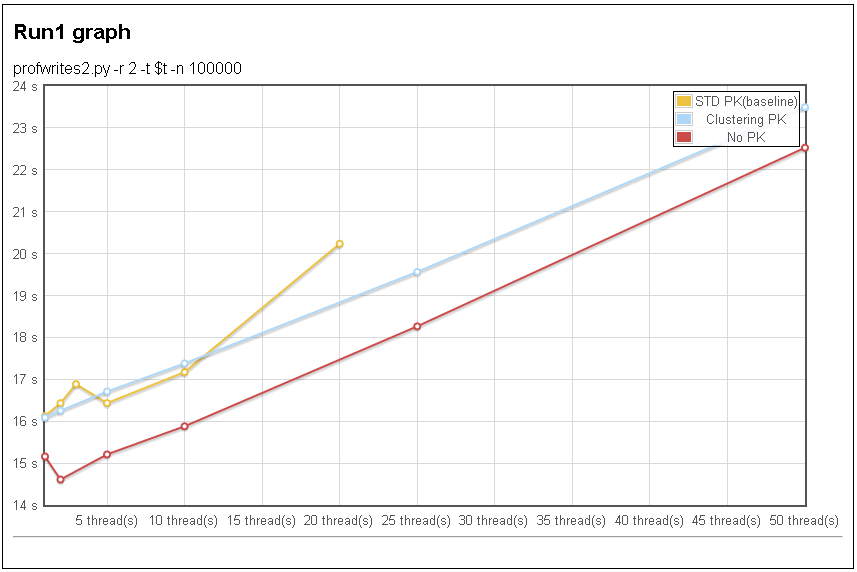
\includegraphics[width=12cm]{assignment2/run1index}
  \caption[Insert performance]{Graph of insert timing for 100.000 rows(in one
  transaction -x1) as a function of concurrency}\label{fig:part1aindex1}
\end{figure}

To support this, this unified diff of DB2 snapshot information illustrates
the difference:
\begin{verbatim}
-Buffer pool index logical reads            = 574013
-Buffer pool index physical reads           = 27
+Buffer pool index logical reads            = 48
+Buffer pool index physical reads           = 23
\end{verbatim}
``-'' prefixes with normal primary key and ``+'' prefixes the snapshot when
inserting into a table without primary key (and thereby without index).

Additionally this can also be seen in the log activity:
\begin{verbatim}
-Log pages written                          = 7708
-Log write time (sec.ns)                    = 23.000000004
-Number write log IOs                       = 1137
+Log pages written                          = 3364
+Log write time (sec.ns)                    = 18.000000004
+Number write log IOs                       = 865
\end{verbatim}

This only means that I've minimized the time spent doing ``superflous''
activity. When loggin at vmstat output, this actually means the we see even less
write activity to the disk with a possibility of writing somewhere around
100times as much data per second before we hit a disk bottleneck.

My best guess in this situation is that the time then is spent doing
housekeeping around table structures. DB2 contains a feature to set a table into
``append mode'' somewhat similar to remove indexes from the table. Maybe
additional performance can be found here?
\begin{figure}
  \centering
  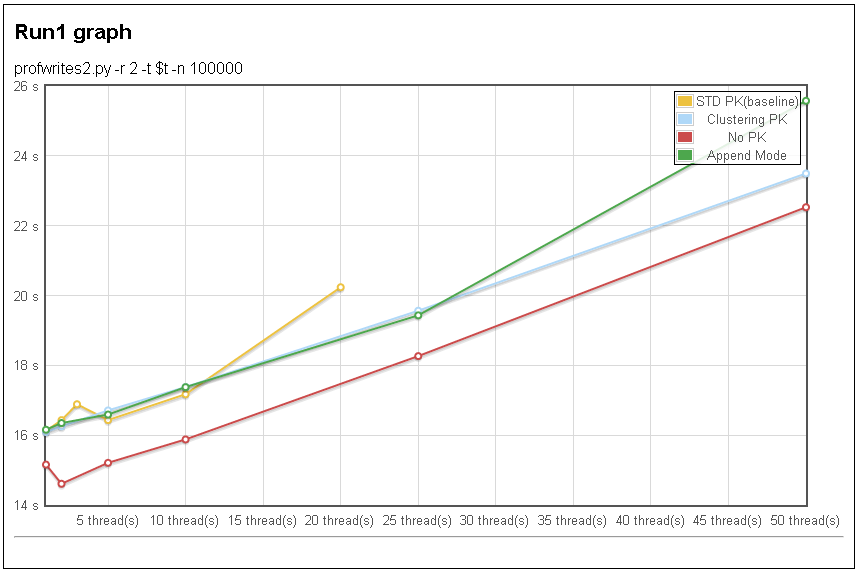
\includegraphics[width=13cm]{assignment2/run1append}
  \caption[Insert performance]{Graph of insert timing for 100.000 rows(in one
  transaction -x1) as a function of concurrency - incl append mode}\label{fig:part1aappnd}
\end{figure}

Figure \ref{fig:part1aappnd} added another line to the graph from figure
\ref{fig:part1aindex1}. No improvement what so ever.

\subsubsection{Log knobs}
Then maybe some database parameters will allow me to speed up insertion rate. I
chose the size of the Log Buffer (LOGBUFSZ) and the Changed Page Threshold.
Firstly a larger buffer will allow me to write more before 


\chapter{Part2}


\chapter{Log book over experiments}

\section{Part 1}

\subsection{Problems with writes.py}\label{log:probwrite}
\begin{itemize}
  \item[2010-03 16-20] Noticed no IO when executing run 2..n of part1a.
    \begin{itemize}
      \item Changed writes.py to use multiprocessing.Pool and allow for writes on
    all runs (Appendix \ref{app:prof}) as well as remove the shared mutex
    between threads there by removing a heavy bottleneck on system level Context
    switches.
   \end{itemize}
  \item Executed 10runs to flatten out any outlieres with amazon ec2 with each
    (Appendix \ref{app:setup})
  \item[2010-03 21] Part1b in the assignement text says that you need to use a \verb|db2 +c|\ldots
    command to enforce a tablelock. That doesnt work because the script uses
    another connection. Changed the script to contain a ``lock table'' part.
    (Included in appendix \ref{app:tl} and was also added to my profwrites2.py
    script).
  \item[2010-04 04] Read newsgroup and read that a bug existed in writes.py
    concerns the ``AUTO\_COMMIT'' parts of the code.\\
    Fixed the script and verified that my old experiments is void:
    \begin{itemize}
      \item Run from 2010-03-20: \verb|Commit statements attempted  = 500037|
      \item Run from 2010-04-04 with fixed script \verb|Commit statements attempted  = 4|
    \end{itemize}
    Notice that the scripts included in the appendix ARE fixed now. 
    This affects all experiments until today, including assignment1.
\end{itemize}

\section{Part2}
\begin{itemize}
  \item part2
\end{itemize}

\appendix
\chapter{Appendix}
\section{Profwrites2.py}\label{app:prof}
New edition of the writes.py that does work on subsequent runs as well as no
shared mutex.
\lstinputlisting{assignment2/profwrites2.py}

\section{writestl.py}\label{app:tl}
New edition of the writes.py that contains a tablelocking switch.
\lstinputlisting{assignment2/writestl.py}

\section{setup.bash and experiment execution}\label{app:setup}
To even out any ec2 glitches I ran the experiements several times:
\begin{verbatim}
$ for i in `seq 3`; 
do 
   echo $i; 
   bash run1.bash; 
   bash run2.bash; 
   bash tl.bash; 
done
\end{verbatim}

\subsection{Tool script included by all experiment specific scripts}
\lstinputlisting{assignment2/setup.bash}

\subsection{Experiment scripts for assignment2-part1}

Part1a:\\
Different threadcounts and index/private key/append mode for tables.
\lstinputlisting{assignment2/run1.bash}
Part1a:\\
Experiment with LOGBUFSZ, CHNGPGS\_THRES values.
\lstinputlisting{assignment2/run2.bash}
Part1b:\\
Tablelocking both insert and updates.
\lstinputlisting{assignment2/tl.bash}

\end{document}
